\documentclass[12pt]{article}
\usepackage{fancyhdr}
\pagestyle{fancy}
\fancyhf{}
\fancyfoot[C]{\thepage}
\fancyfoot[L]{\scriptsize CC BY-NC-SA 4.0 \textbullet\ Leo Liang}
\renewcommand{\headrulewidth}{0pt}
\usepackage[margin=1in]{geometry}
\usepackage{amsmath, amssymb}
\usepackage{array, booktabs}
\usepackage{pgffor}
\usepackage{tikz}
\parindent=0pt
\parskip=1em
\newcolumntype{C}[1]{>{\centering\arraybackslash}p{#1}}
\newcommand{\wl}{\par\vspace{5mm}\noindent\rule{\linewidth}{0.4pt}\par\vspace{1mm}}
\newcommand{\wls}[1]{\foreach \i in {1,...,#1}{\wl}}
\newcommand{\blk}{\rule[-2pt]{2.2cm}{0.4pt}} % an inline answer blank
% ─────────────────────────────────────────────────────────────────────────────
\begin{document}
\pagestyle{fancy}
\begin{center}
  {\Large\bfseries Homework 5}\\[4pt]
  Algebra Fluency: Distributing \& Combining\\[6pt]
  Name:\;\underline{\hspace{6.5cm}}\quad
\end{center}
\hrule\bigskip

\section*{Instructions}
This homework will prepare you for the next stretch of calculus. Write
your questions in the margin in a different color. You may use AI as a
\textbf{teacher} (ask it to explain or give more examples), but do the problems yourself first.

% ===========================================================================
\section*{Reading 1 --- The Distributive Property}
To \textbf{distribute} means to multiply a factor on the outside of a parenthesis by \emph{every} term on the
inside:
\[
  a(b + c) = ab + ac.
\]
\textbf{Why it works --- think of area.} A rectangle that is $a$ tall and $(b+c)$ wide can be split into two
smaller rectangles. Its total area is the sum of the two pieces:

\begin{center}
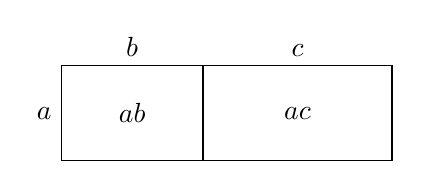
\begin{tikzpicture}[scale=0.6]
  \draw (0,0) rectangle (3,2);
  \draw (3,0) rectangle (7,2);
  \node at (1.5,1) {$ab$};
  \node at (5,1) {$ac$};
  \node[above] at (1.5,2) {$b$};
  \node[above] at (5,2) {$c$};
  \node[left] at (0,1) {$a$};
\end{tikzpicture}
\end{center}

The one rule: the outside factor hits \textbf{each} inside term. For example, $2(x+12)$ is a $2$-tall rectangle of
width $(x+12)$:

\begin{center}
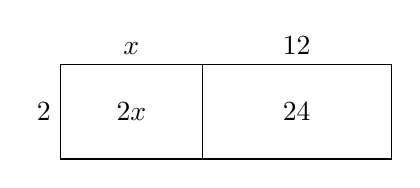
\begin{tikzpicture}[scale=0.6]
  \draw (0,0) rectangle (3,2);
  \draw (3,0) rectangle (7,2);
  \node at (1.5,1) {$2x$};
  \node at (5,1) {$24$};
  \node[above] at (1.5,2) {$x$};
  \node[above] at (5,2) {$12$};
  \node[left] at (0,1) {$2$};
\end{tikzpicture}
\end{center}
so $\;2(x+12) = 2x + 24$. Another: $\;3(2x+5) = 6x + 15$.

\textbf{The tricky part: negatives.} The sign on the outside travels onto \emph{every} inside term.
\[
  -(x+12) = -x - 12, \qquad 2(x-5) = 2x - 10, \qquad -3(2x-4) = -6x + 12.
\]
In the last one, the $-3$ times the $-4$ gives $+12$ --- two negatives make a positive. \textbf{Watch the signs:
that is where most mistakes happen.}

\bigskip
\textbf{Q1.}\quad Distribute each. 

\medskip
\textbf{(a)}\quad $2(x+3) = \blk$ \hfill
\textbf{(b)}\quad $5(x-1) = \blk$

\medskip
\textbf{(c)}\quad $-(x+4) = \blk$ \hfill
\textbf{(d)}\quad $-2(x-6) = \blk$

\medskip
\textbf{(e)}\quad $3(2x+5) = \blk$ \hfill
\textbf{(f)}\quad $-4(3x-2) = \blk$

\medskip
\textbf{(g)}\quad $-(-x+7) = \blk$ \hfill
\textbf{(h)}\quad $-5(2-3x) = \blk$

% ===========================================================================
\newpage
\section*{Reading 2 --- Combining Like Terms}
\textbf{Like terms} have the \emph{same variable part} --- the same letter raised to the same power. You can add
or subtract like terms by combining their coefficients; unlike terms cannot be combined.
\[
  3x + 5x = 8x, \qquad 7x - 2x = 5x, \qquad 4x - 9x = -5x.
\]
But $\;3x$ and $3x^2$ are \textbf{not} like terms (different powers), and $\;3x$ and $7$ are \textbf{not} like
terms (one has $x$, one does not). Watch the signs again: $4x - 9x = -5x$, not $5x$.

\textbf{Putting it together: distribute, then combine.}
\[
  2(x+3) + 4x = 2x + 6 + 4x = 6x + 6.
\]

\bigskip
\textbf{Q2.}\quad Combine the like terms.

\medskip
\textbf{(a)}\quad $3x + 5x = \blk$ \hfill
\textbf{(b)}\quad $4x - 9x = \blk$

\medskip
\textbf{(c)}\quad $3x + 7 + 2x - 1 = \blk$ \hfill
\textbf{(d)}\quad $5x - 3 - 8x + 6 = \blk$

\bigskip
\textbf{Q3.}\quad Distribute, then combine like terms.

\medskip
\textbf{(a)}\quad $2(x+3) + 4x$
\wl

\textbf{(b)}\quad $-2(x-5) + 3x$
\wl

\textbf{(c)}\quad $4(2x+1) - 3(x-2)$
\wl

% ===========================================================================
\newpage
\section*{Application --- Areas and Catching Mistakes}
\textbf{Two-term products with the area model.} To multiply $(x+3)(x+2)$, make a rectangle that is $(x+3)$ wide and
$(x+2)$ tall, and split each side. Every piece of area is one product; add them all up.

\begin{center}
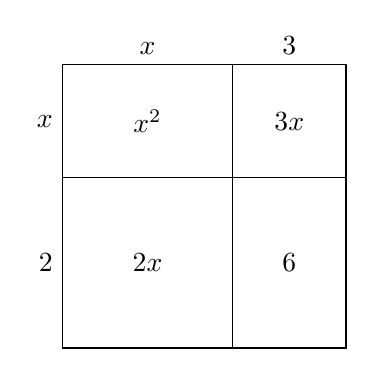
\begin{tikzpicture}[scale=0.9]
  \draw (0,0) rectangle (4,4);
  \draw (2.4,0)--(2.4,4);
  \draw (0,2.4)--(4,2.4);
  \node at (1.2,3.2) {$x^2$};
  \node at (3.2,3.2) {$3x$};
  \node at (1.2,1.2) {$2x$};
  \node at (3.2,1.2) {$6$};
  \node[above] at (1.2,4) {$x$};
  \node[above] at (3.2,4) {$3$};
  \node[left] at (0,3.2) {$x$};
  \node[left] at (0,1.2) {$2$};
\end{tikzpicture}
\end{center}
Adding the four pieces: $(x+3)(x+2) = x^2 + 3x + 2x + 6 = x^2 + 5x + 6$.

\bigskip
\textbf{Q4.}\quad \textbf{Minecraft floor.} A room is $(x+5)$ blocks wide and $(x+2)$ blocks long. Fill in the area
box, then write the total floor area as a single expanded expression.

\begin{center}
\begin{tikzpicture}[scale=0.9]
  \draw (0,0) rectangle (4,4);
  \draw (2.2,0)--(2.2,4);
  \draw (0,2.2)--(4,2.2);
  \node[above] at (1.1,4) {$x$};
  \node[above] at (3.1,4) {$5$};
  \node[left] at (0,3.1) {$x$};
  \node[left] at (0,1.1) {$2$};
\end{tikzpicture}
\end{center}
Total floor area $= \blk\blk$

\bigskip
\textbf{Q5.}\quad \textbf{Spot the error.} Each line below has a mistake. Find it, say what went wrong in a few
words, and write the correct answer.

\medskip
\textbf{(a)}\quad $-2(x-5) = -2x - 10$
\wl

\textbf{(b)}\quad $3(x+4) = 3x + 4$
\wl

\textbf{(c)}\quad $5x - 8x = 3x$
\wl

\textbf{(d)}\quad $-(x-7) = -x - 7$
\wl

% ===========================================================================
\newpage
\section*{$\bigstar$ Going Further (stretch)}
\textit{This section is a stretch --- give it a real try, and do not worry if you do not finish.}

\textbf{Squaring a sum.} The area model also expands $(x+h)^2$ --- a square that is $(x+h)$ on each side:

\begin{center}
\begin{tikzpicture}[scale=0.9]
  \draw (0,0) rectangle (4,4);
  \draw (2.6,0)--(2.6,4);
  \draw (0,2.6)--(4,2.6);
  \node[above] at (1.3,4) {$x$};
  \node[above] at (3.3,4) {$h$};
  \node[left] at (0,3.3) {$x$};
  \node[left] at (0,1.3) {$h$};
\end{tikzpicture}
\end{center}

\textbf{Q6.}\quad (a) Fill in the four pieces of the square above, then write $(x+h)^2$ as an expanded expression.
\wl
(b) Use it (or multiply it out) to expand $(x+h)^3 = (x+h)(x+h)^2$.
\wls{2}

\bigskip
\textbf{Q7.}\quad \textbf{A tough simplification.}\quad Simplify this expression completely. Use your expansion of
$(x+h)^2$ from Q6.
\[
  \frac{(x+h)^2 - x^2}{h}.
\]


\end{document}